\documentclass[a4paper, 9pt]{jsarticle}
%マージンの設定
\usepackage[top=20mm, bottom=20mm, left=20mm, right=20mm]{geometry}
%フォントの設定(セリフ体がカッコ悪いので)
\usepackage[T1]{fontenc}
\usepackage[scaled]{helvet}
\usepackage{graphicx}
\usepackage{here}
%単位
\newcommand{\ut}[1]{\;\mbox{$\mathrm{#1}$}}


%タイトルに書きたいことを書く
\title{\textbf{基礎科学実験C 実験レポート}}
\author{学籍番号 9999999\\こねこ。}
\date{\today 提出}

\begin{document}
\maketitle

※ここに書かれている実験は仮想的なものです.実際には行っていません.したがって,内容に関する物理学的正しさは保証しません.
\section{目的}
この実験では,ピアノから発せられる「A4」に該当する音の周波数を求める.

\section{原理}
正弦進行波
\begin{equation}
  u_1(x, t) = A\sin{(k_1x - \omega_1 t)}
\end{equation}
\begin{equation}
  u_2(x, t) = A\sin{(k_2x - \omega_2 t)}
\end{equation}
を重ね合わせるとする.このとき,

\begin{equation}
  \Delta \omega = \omega_1 - \omega_2,\quad\displaystyle\omega = \frac{\omega_1 + \omega_2}{2}
\end{equation}
\begin{equation}
  \Delta k = k_1 - k_2,\quad\displaystyle k = \frac{k_1 + k_2}{2}
\end{equation}
を定義する.ここで,$\Delta \omega \ll \omega$および$\Delta k \ll k$であるとする.合成波は
\begin{equation}
  u(x, t) = 2A\cos{\left(\frac{\Delta k}{2}x - \frac{\Delta \omega}{2}t\right)}\sin{\left(kx - \omega t\right)}
\end{equation}
となり,この新服は時間的・空間的にゆっくりと変化する.その包絡線は,
\begin{equation}
  \pm \left|2A\cos{\left(\frac{\Delta k}{2}x - \frac{\Delta \omega}{2}t\right)}\right|
\end{equation}
により表され,包絡線自体も波を形成する.このような波をうなりという.\par
この実験では,このうなりの周期がゼロになる点を探す.

\section{実験}
この実験は,ピアノとスマートフォンを用いておこなった.図\ref{fig1}のように,電子ピアノのA4キーにおもりを取り付け,音を鳴らし続けた.はじめ,スマートフォンからは$440\ut{Hz}$の音を出力した.次に,スマートフォンから出力される音を$300\ut{Hz}$までゆっくりと変化させ,うなりが消えた瞬間があれば,その周波数を記録した.次に,スマートフォンから出力される音を$500\ut{Hz}$までゆっくりと変化させ,うなりが消えた瞬間があれば,その周波数を記録した.以上の操作を5回行った.
\begin{figure}[H]
  \centering
  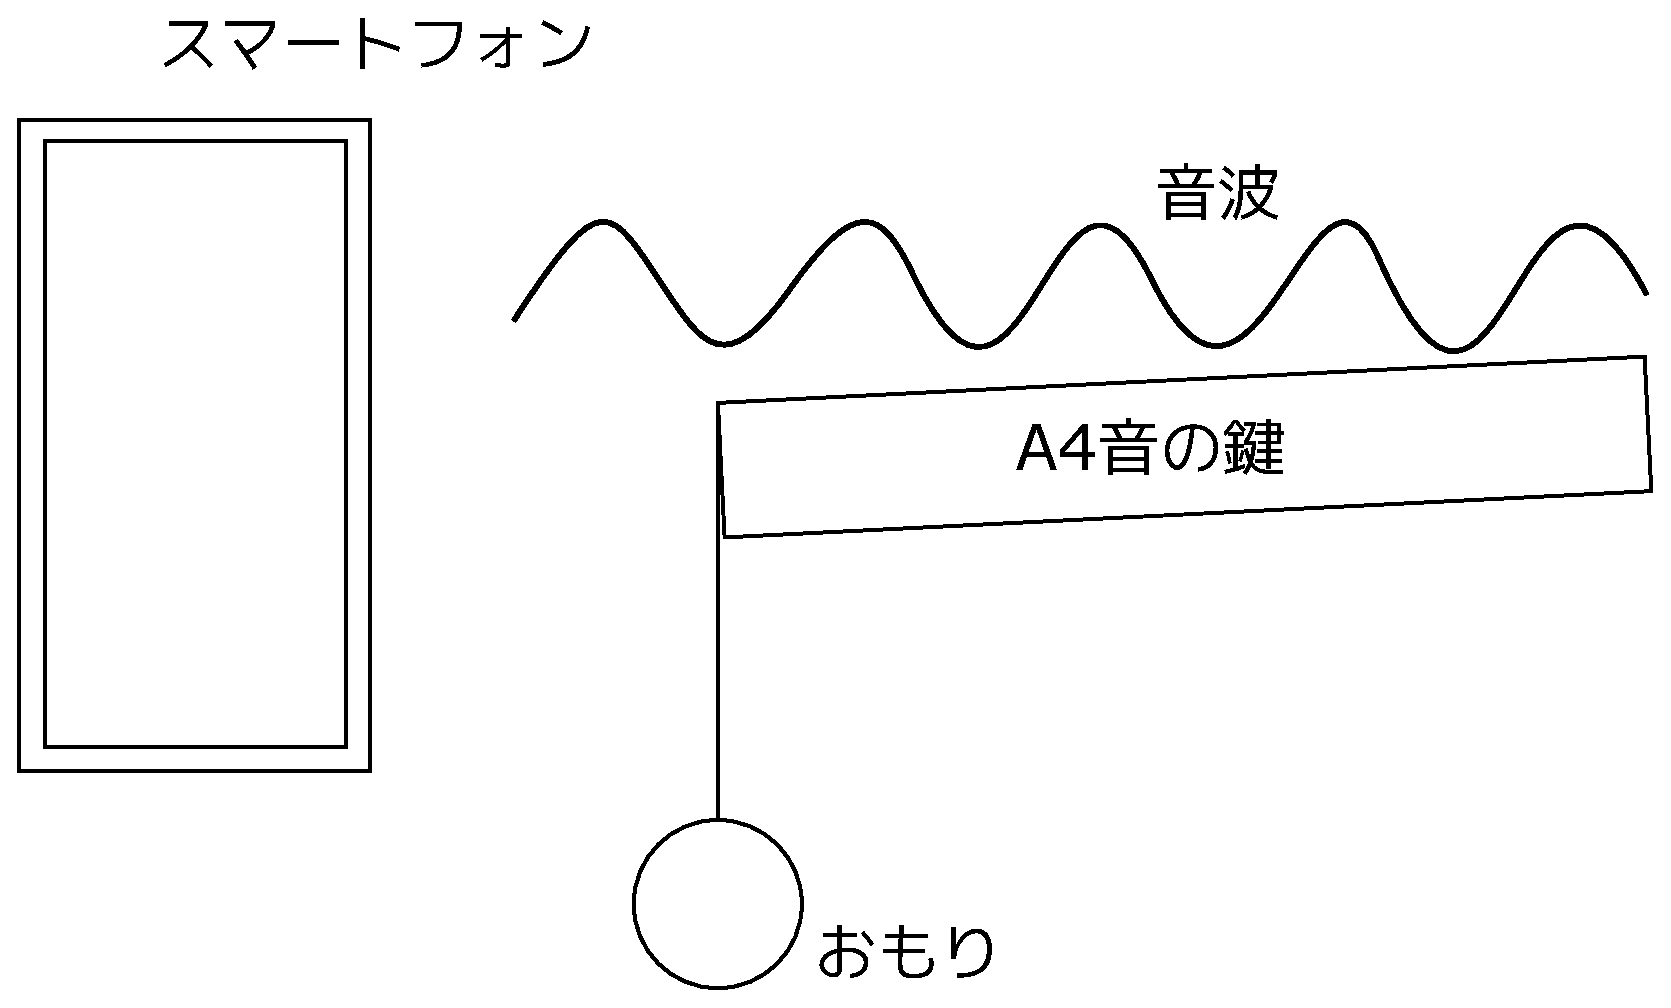
\includegraphics[scale=0.2]{fig.eps}
  \caption{実験装置の図}
  \label{fig1}
\end{figure}

\section{結果}
結果は表\ref{tab1}のようになった.
\begin{table}[H]
  \centering
  \caption{実験結果}
  \begin{tabular}{c}
    \hline
    測定した周波数$f/\mathrm{Hz}$ \\
    \hline
    442                           \\
    440                           \\
    439                           \\
    441                           \\
    440                           \\
    \hline
  \end{tabular}
  \label{tab1}
\end{table}

平均値$\bar{f}$は,以下のように算出した.ただし,途中式の単位は省略した.
\[\bar{f} = \frac{1}{5}(442 + 440 + 439 + 441 + 440) = 440.4 \ut{Hz}\]
平均値$\bar{f}$の標準不確かさ$\Delta \bar{f}$は,以下のように算出した.ただし,途中式の単位は省略した.
\[\Delta \bar{f} = \sqrt{\frac{1}{5\cdot(5-1)}\{(442 - 440.4)^2 + (440 - 440.4)^2 + (439 - 440.4)^2 + (441 - 440.4)^2 + (440 - 440.4)^2\} } \simeq 0.51\ut{Hz}\]
測定値の有効数字は3桁であるから,$\bar{f} = 440\ut{Hz}$であり,$\bar{f}$の最小桁に合わせると$\Delta \bar{f} = 1\ut{Hz}$である.
\begin{table}[H]
  \centering
  \caption{実験結果の平均値とその不確かさ}
  \begin{tabular}{c}
    \hline
    測定した周波数の平均値$\bar{f}/\mathrm{Hz}$ \\
    \hline
    $440 \pm 1$                                 \\
    \hline
  \end{tabular}
  \label{tab2}
\end{table}

\section{考察}
周波数は文献値$440\ut{Hz}$に一致した.これほど精度の高い値が得られた理由は,前日に調律をしたことによる.通常,調律においては本実験におけるプロセスとほぼ同様の手法を用いて音合わせを行う.うなりの回数を$\Delta f$,調律前のA4音の周波数を$f_1$とすると,
\begin{equation}
  |f_1 - 440\ut{Hz}| = \Delta f
\end{equation}
である.ピアノの調律においてもiPhoneやiPadでインストールできるチューナーを用いることが多く,実験と同様のプロセスで調律が行われる.$\Delta f$に含まれる誤差が調律で用いるスマートフォンと今回実験で用いたスマートフォンとで有意差を生じなかったことにより,本実験においては精度の高い実験結果が得られた.


% 参考文献
\begin{thebibliography}{99}
  \bibitem{nami} 伊東敏雄,“な〜るほど!の波と光”,学術図書出版,1997-4-20発行,pp.11-14, pp.46-58
\end{thebibliography}

\end{document}